% Slide deck explaining the model. Built once with:
%   cd docs/model && pdflatex model.tex && pdflatex model.tex && cp model.pdf ../../model.pdf
\documentclass[aspectratio=169,11pt]{beamer}

\usepackage{amsmath,amssymb}
\usepackage[normalem]{ulem}
\usepackage{tikz}
\usepackage{pgfplots}
\pgfplotsset{compat=1.18}
\usepgfplotslibrary{fillbetween}
\usetikzlibrary{positioning,fit,arrows.meta,backgrounds,shapes.geometric}

\definecolor{ink}{HTML}{16222C}
\definecolor{accent}{HTML}{1F77B4}
\definecolor{good}{HTML}{2E8B57}
\definecolor{warn}{HTML}{C0392B}
\definecolor{amber}{HTML}{D68910}
\definecolor{muted}{HTML}{7A8894}
\definecolor{wash}{HTML}{EFF3F6}

\usetheme{default}
\usecolortheme{default}
\setbeamertemplate{navigation symbols}{}
\setbeamercolor{structure}{fg=accent}
\setbeamercolor{normal text}{fg=ink}
\setbeamercolor{frametitle}{fg=ink}
\setbeamerfont{frametitle}{size=\Large,series=\bfseries}
\setbeamerfont{title}{size=\huge,series=\bfseries}
\setbeamertemplate{itemize item}{\color{accent}\rule[0.35ex]{0.5em}{0.5em}}
\setbeamertemplate{itemize subitem}{\color{muted}\rule[0.35ex]{0.35em}{0.35em}}
\setbeamertemplate{frametitle}{%
  \vspace{0.7em}\hspace{0.9em}\insertframetitle%
  \vspace{0.15em}\newline\hspace*{0.9em}%
  {\color{accent}\rule{2.2em}{2.2pt}}\vspace{0.2em}}
\setbeamertemplate{footline}{%
  \hfill{\color{muted}\scriptsize\insertframenumber\hspace{1.2em}}\vspace{0.5em}}

\newcommand{\lead}[1]{{\color{accent}\bfseries #1}}
\newcommand{\bad}[1]{{\color{warn}\bfseries #1}}
\newcommand{\ok}[1]{{\color{good}\bfseries #1}}

% A key-number callout: big figure, small caption underneath.
\newcommand{\stat}[3]{%
  \begin{minipage}[t]{#1}\centering
  {\fontsize{20}{22}\selectfont\bfseries\color{accent}#2}\\[0.25em]
  {\scriptsize\color{muted}#3}
  \end{minipage}}

\title{How fast does the market\\price in the news?}
\subtitle{}
\date{}
\author{}

\begin{document}

% ---------------------------------------------------------------- title
{\setbeamertemplate{footline}{}
\begin{frame}[plain]
\vspace{1.2em}
\begin{center}
{\fontsize{34}{40}\selectfont\bfseries How fast does the market\\[0.2em] price in the news?}\\[1.6em]
{\large\color{muted} A measurement study. Not a strategy.}\\[2.2em]
{\color{accent}\rule{6em}{2.5pt}}\\[1.6em]
{\small\color{muted}\texttt{proj-price-discovery}\quad$\cdot$\quad the model in 14 slides}
\end{center}
\end{frame}}

% ---------------------------------------------------------------- 1
\begin{frame}{The setup}
\vspace{0.6em}
\begin{columns}[T,onlytextwidth]
\begin{column}{0.52\textwidth}
\begin{itemize}\setlength\itemsep{0.9em}
\item CPI lands at \lead{08:30:00 ET}, to the second
\item Nobody knows the number one second earlier
\item Crypto trades \lead{24/7} --- no auction, no open
\end{itemize}
\vspace{1.2em}
{\color{muted}So the release is a clean shock into a live market.}
\end{column}
\begin{column}{0.44\textwidth}
\centering
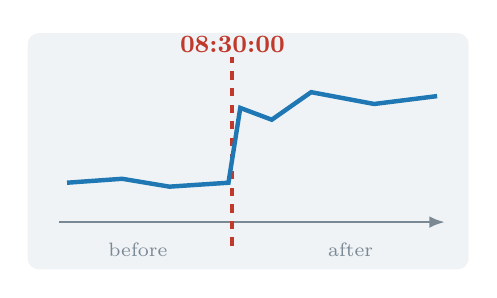
\begin{tikzpicture}[font=\small]
\fill[wash,rounded corners] (-0.2,-1.5) rectangle (5.4,1.5);
\draw[muted,line width=1pt,-{Latex[length=2mm]}] (0.2,-0.9) -- (5.1,-0.9);
\draw[warn,line width=1.4pt,dashed] (2.4,-1.2) -- (2.4,1.2);
\node[warn,font=\small\bfseries] at (2.4,1.35) {08:30:00};
\draw[accent,line width=1.6pt]
  (0.3,-0.4) -- (1.0,-0.35) -- (1.6,-0.45) -- (2.35,-0.4)
  -- (2.5,0.55) -- (2.9,0.4) -- (3.4,0.75) -- (4.2,0.6) -- (5.0,0.7);
\node[muted,font=\scriptsize] at (1.2,-1.25) {before};
\node[muted,font=\scriptsize] at (3.9,-1.25) {after};
\end{tikzpicture}
\end{column}
\end{columns}
\end{frame}

% ---------------------------------------------------------------- 2
\begin{frame}{Does it even react? We checked first.}
\vspace{-1.0em}
\begin{center}
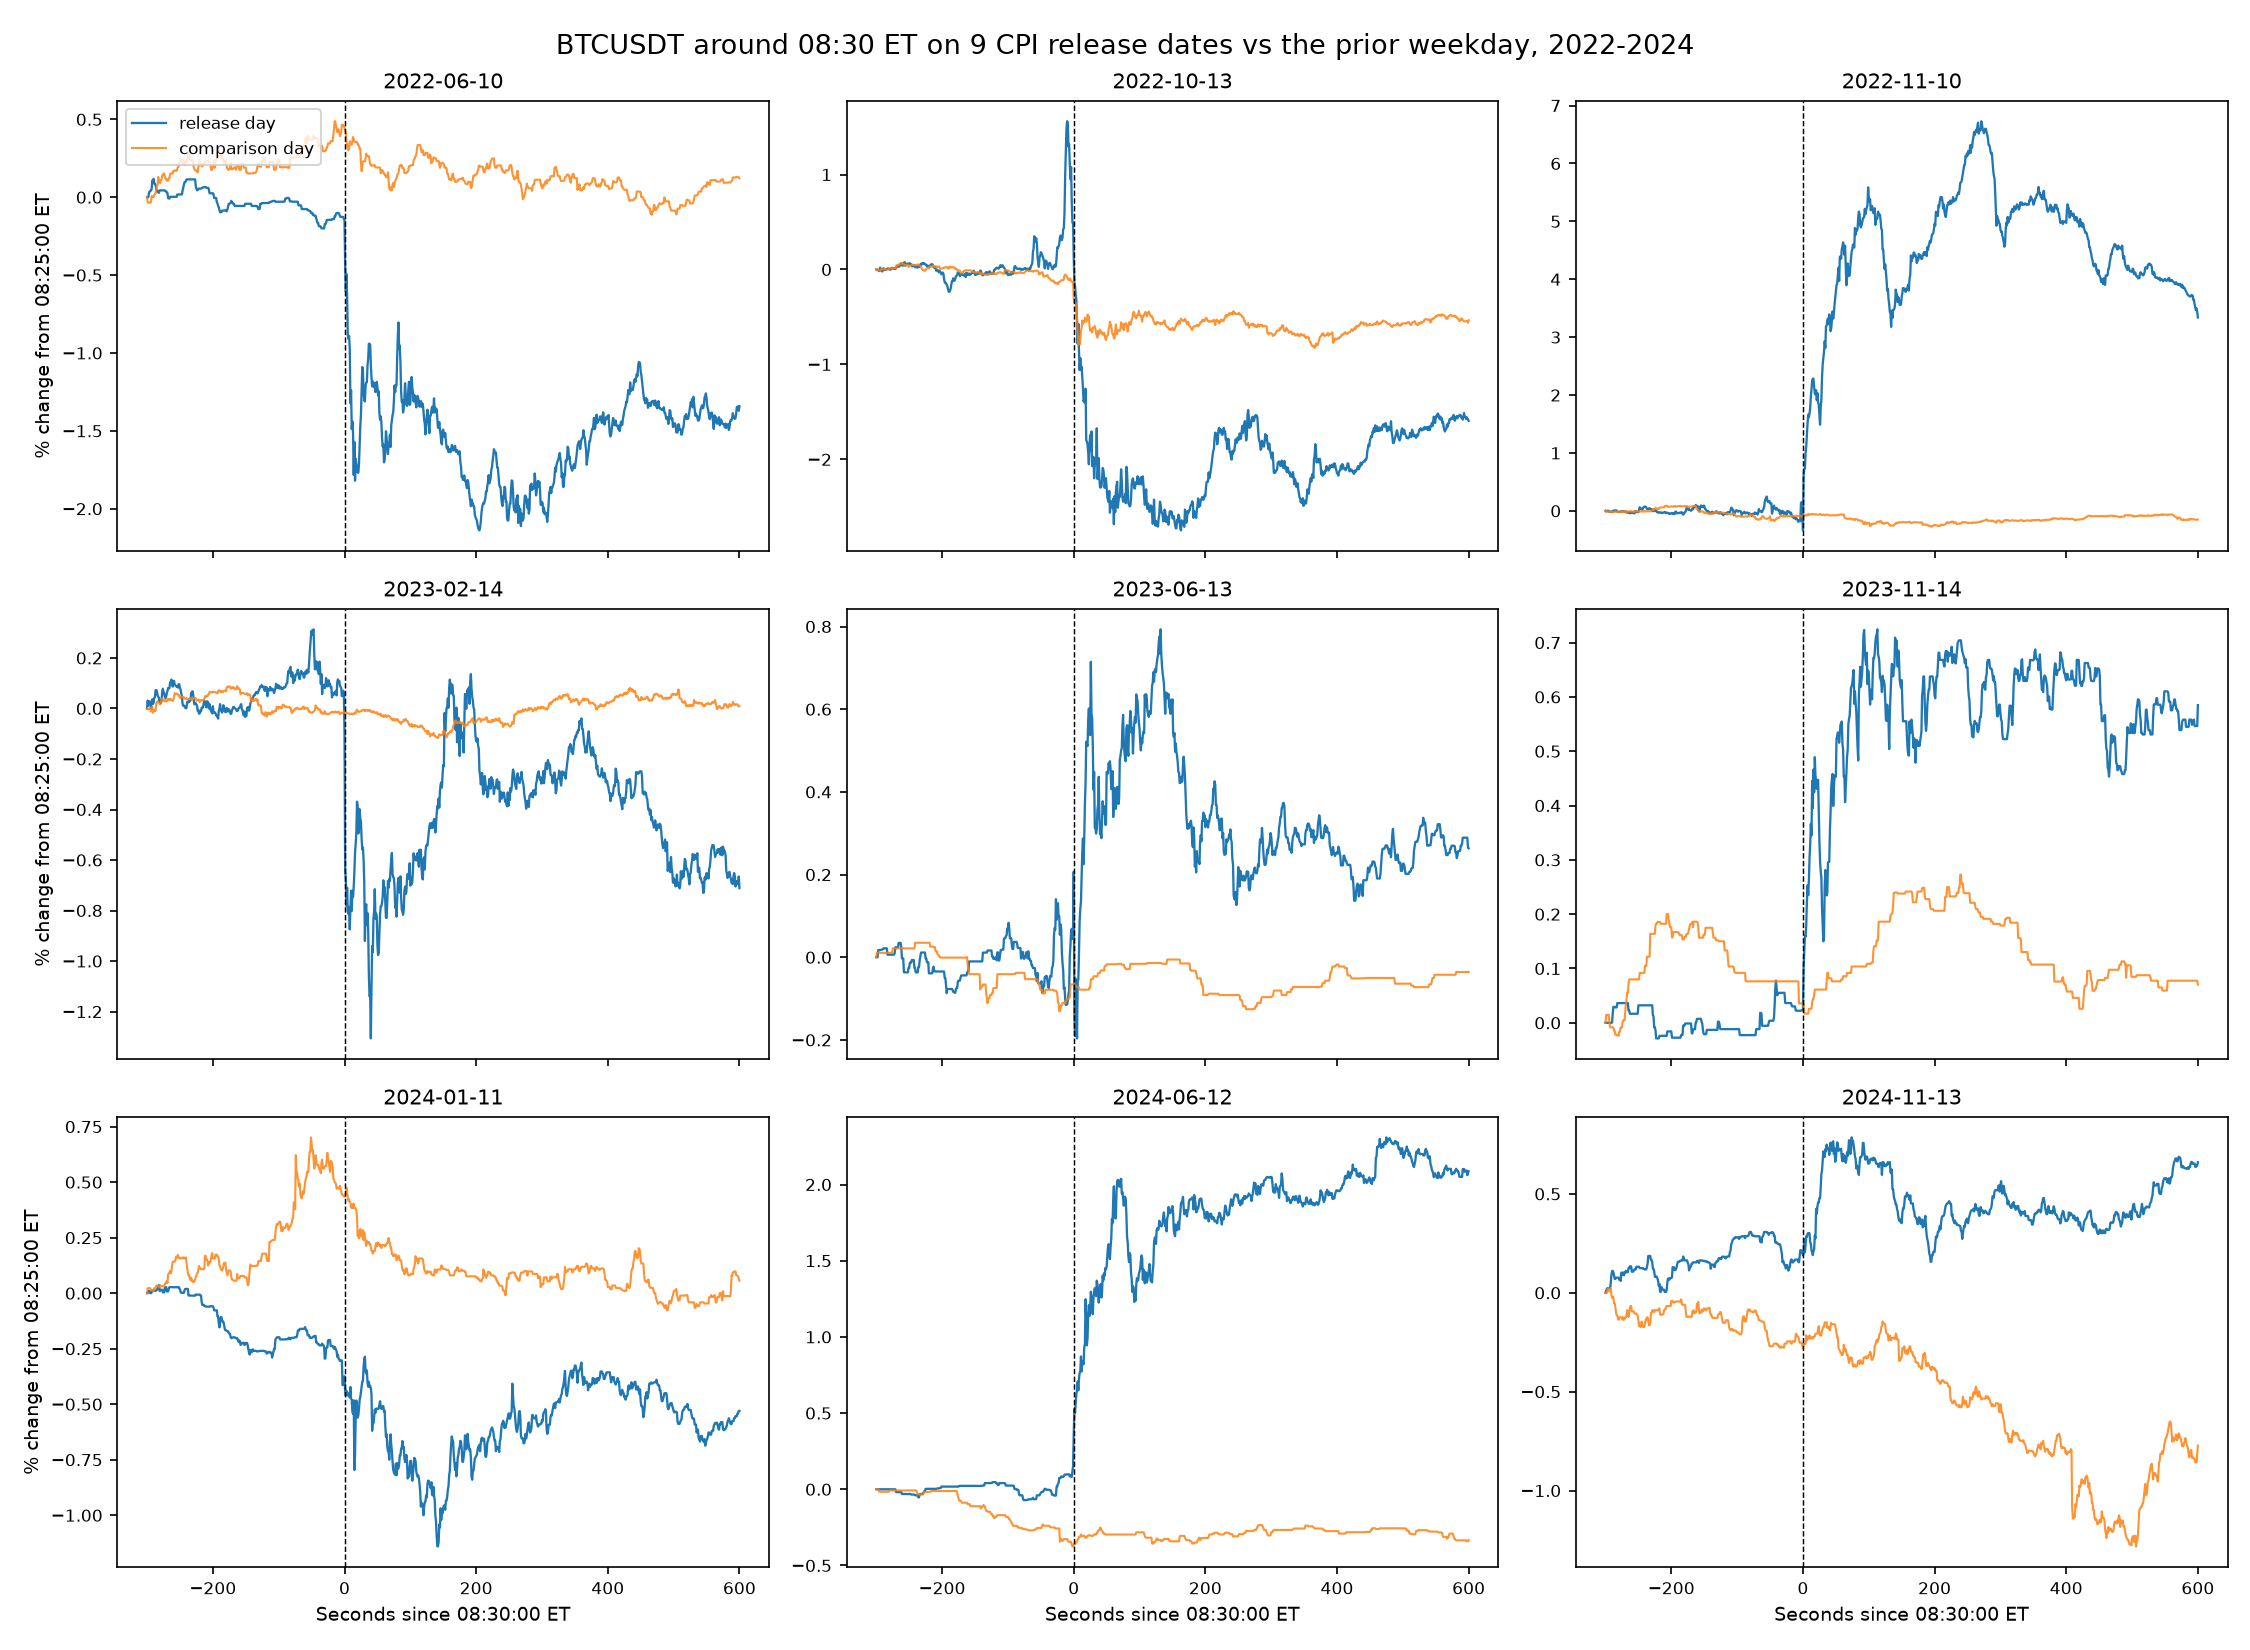
\includegraphics[height=0.57\textheight]{../../figures/spikeGrid.png}
\end{center}
\vspace{0.1em}
\begin{center}
\stat{0.28\textwidth}{9 / 9}{dates show a jump}\hfill
\stat{0.28\textwidth}{5.6$\times$}{median vs.\ a normal day}\hfill
\stat{0.28\textwidth}{$\pm$}{sign follows the surprise}
\end{center}
\end{frame}

% ---------------------------------------------------------------- 3
\begin{frame}{The question, made precise}
\vspace{1.4em}
\begin{center}
{\fontsize{22}{26}\selectfont
Of the move the release eventually causes,\\[0.5em]
\lead{what fraction has happened by} $\boldsymbol\tau$ \lead{seconds?}}
\end{center}
\vspace{1.8em}
\begin{center}
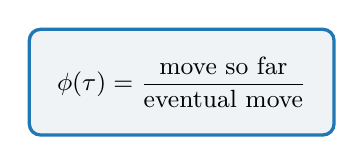
\begin{tikzpicture}[font=\small]
\node[draw=accent,line width=1.2pt,rounded corners,fill=wash,inner sep=10pt]
  {$\displaystyle \phi(\tau)=\frac{\text{move so far}}{\text{eventual move}}$};
\end{tikzpicture}
\end{center}
\vspace{1.4em}
\begin{center}
{\color{muted}Report it at 1\,s, 10\,s, 1\,min, 10\,min, 1\,h. One curve.}
\end{center}
\end{frame}

% ---------------------------------------------------------------- 4
\begin{frame}{What the curve looks like}
\vspace{-0.3em}
\begin{columns}[T,onlytextwidth]
\begin{column}{0.58\textwidth}
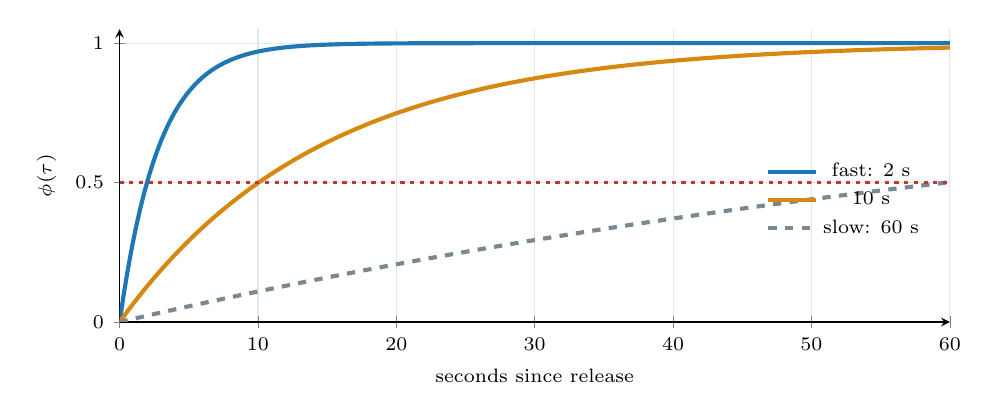
\begin{tikzpicture}
\begin{axis}[
  width=\textwidth, height=5.3cm,
  xlabel={seconds since release}, ylabel={$\phi(\tau)$},
  xmin=0,xmax=60,ymin=0,ymax=1.05, ytick={0,0.5,1},
  grid=major, grid style={muted!20}, axis lines=left,
  every axis plot/.append style={line width=1.5pt},
  legend style={draw=none,fill=none,font=\scriptsize,at={(0.98,0.25)},anchor=south east},
  tick label style={font=\scriptsize}, label style={font=\scriptsize},
]
\addplot[accent,domain=0:60,samples=200]{1-exp(-0.35*x)};  \addlegendentry{fast: 2 s}
\addplot[amber,domain=0:60,samples=200]{1-exp(-0.069*x)};  \addlegendentry{10 s}
\addplot[muted,dashed,domain=0:60,samples=200]{1-exp(-0.0116*x)}; \addlegendentry{slow: 60 s}
\addplot[warn,dotted,line width=1pt,domain=0:60]{0.5};
\end{axis}
\end{tikzpicture}
\end{column}
\begin{column}{0.38\textwidth}
\vspace{0.8em}
$$\phi(\tau)=\frac{1-e^{-\lambda\tau}}{1-e^{-\lambda H}}$$
\vspace{0.1em}

One number per event: \lead{$\lambda$},\\
reported as the time to get halfway
$$\tau_{1/2}=\frac{1}{\lambda}\ln\frac{2}{1+e^{-\lambda H}}$$
\vspace{-0.2em}

{\color{muted}\small ``half the move happened in 6.9 seconds'' --- a sentence you can argue with.}
\end{column}
\end{columns}
\end{frame}

% ---------------------------------------------------------------- 5
\begin{frame}{The obvious way to compute it}
\vspace{1.0em}
\begin{center}
{\large For each event, divide. Then average.}
\end{center}
\vspace{1.2em}
\begin{center}
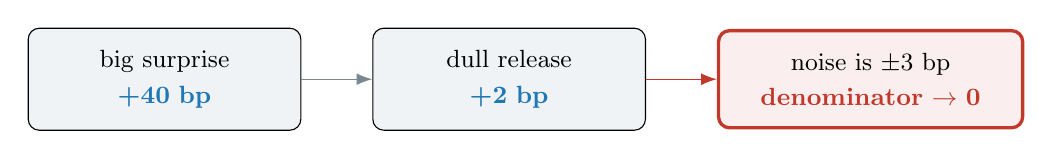
\begin{tikzpicture}[font=\small,node distance=0.9cm]
\node[draw,rounded corners,fill=wash,inner sep=8pt,text width=2.9cm,align=center] (a)
  {big surprise\\[0.2em]\lead{+40 bp}};
\node[draw,rounded corners,fill=wash,inner sep=8pt,text width=2.9cm,align=center,right=of a] (b)
  {dull release\\[0.2em]\lead{+2 bp}};
\node[draw=warn,line width=1.2pt,rounded corners,fill=warn!8,inner sep=8pt,text width=3.3cm,align=center,right=of b] (c)
  {noise is $\pm$3 bp\\[0.2em]\bad{denominator $\to$ 0}};
\draw[-{Latex[length=2mm]},muted] (a)--(b);
\draw[-{Latex[length=2mm]},warn] (b)--(c);
\end{tikzpicture}
\end{center}
\vspace{1.4em}
\begin{center}
\bad{One event can flip the average.}
\end{center}
\end{frame}

% ---------------------------------------------------------------- 6
\begin{frame}{The usual fix is the real trap}
\vspace{1.6em}
\begin{center}
{\large ``Just drop the events where the price barely moved.''}
\end{center}
\vspace{1.8em}
\begin{center}
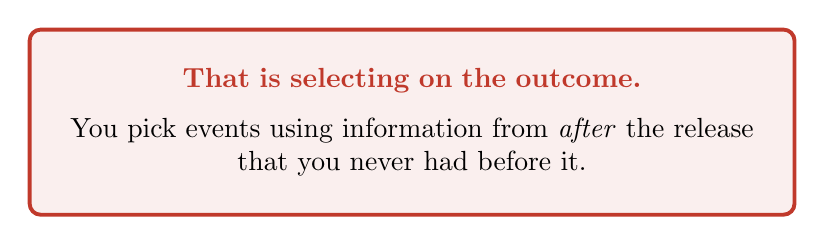
\begin{tikzpicture}
\node[draw=warn,line width=1.4pt,rounded corners,fill=warn!8,inner sep=14pt,text width=0.72\textwidth,align=center]
  {\bad{That is selecting on the outcome.}\\[0.6em]
   You pick events using information from \emph{after} the release\\
   that you never had before it.};
\end{tikzpicture}
\end{center}
\vspace{1.4em}
\begin{center}
{\color{muted}The fastest route to a clean-looking wrong answer,\\
and the first thing a reviewer looks for.}
\end{center}
\end{frame}

% ---------------------------------------------------------------- 7
\begin{frame}{So we never divide}
\vspace{0.5em}
\begin{center}
{\large Give every event \lead{two} parameters instead of one.}
\end{center}
\vspace{0.7em}
\begin{center}
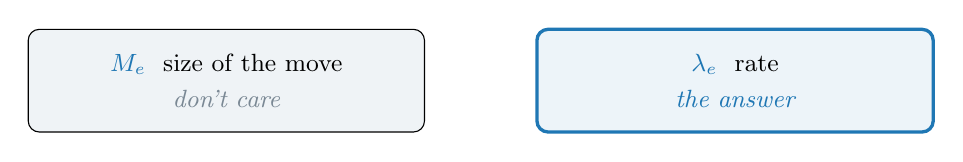
\begin{tikzpicture}[font=\small]
\node[draw,rounded corners,fill=wash,inner sep=9pt,text width=4.4cm,align=center] (A)
  {\lead{$M_e$}\ \ size of the move\\[0.2em]{\color{muted}\itshape don't care}};
\node[draw=accent,line width=1.2pt,rounded corners,fill=accent!8,inner sep=9pt,text width=4.4cm,align=center,right=1.4cm of A] (L)
  {\lead{$\lambda_e$}\ \ rate\\[0.2em]{\color{accent}\itshape the answer}};
\end{tikzpicture}
\end{center}
\vspace{0.6em}
$$m_e(\tau)=M_e\,\frac{1-e^{-\lambda_e\tau}}{1-e^{-\lambda_e H}}
\qquad\Longrightarrow\qquad
\phi_e(\tau)=\frac{1-e^{-\lambda_e\tau}}{1-e^{-\lambda_e H}}$$
\vspace{0.1em}
\begin{center}
\ok{The size cancels.} A dull event now gives a \emph{wide} answer\\
{\color{muted}instead of a divergent one. Nothing is dropped.}
\end{center}
\end{frame}

% ---------------------------------------------------------------- 8
\begin{frame}{214 events. Now what?}
\vspace{0.6em}
\begin{center}
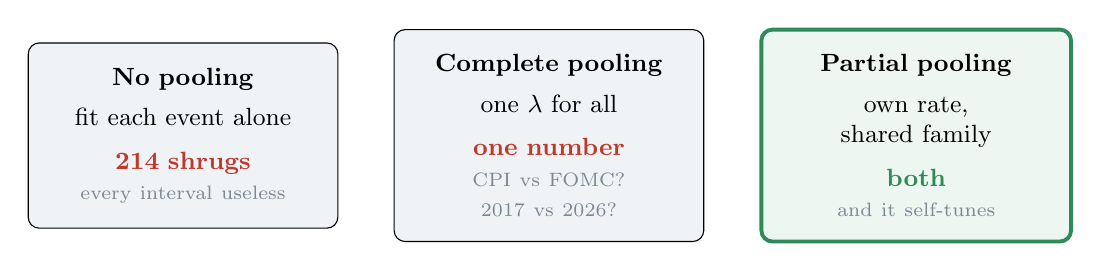
\begin{tikzpicture}[font=\small]
\node[draw,rounded corners,fill=wash,inner sep=9pt,text width=3.3cm,align=center] (n)
  {\textbf{No pooling}\\[0.4em]fit each event alone\\[0.5em]\bad{214 shrugs}\\{\color{muted}\scriptsize every interval useless}};
\node[draw,rounded corners,fill=wash,inner sep=9pt,text width=3.3cm,align=center,right=0.7cm of n] (c)
  {\textbf{Complete pooling}\\[0.4em]one $\lambda$ for all\\[0.5em]\bad{one number}\\{\color{muted}\scriptsize CPI vs FOMC? 2017 vs 2026?}};
\node[draw=good,line width=1.4pt,rounded corners,fill=good!8,inner sep=9pt,text width=3.3cm,align=center,right=0.7cm of c] (p)
  {\textbf{Partial pooling}\\[0.4em]own rate, shared family\\[0.5em]\ok{both}\\{\color{muted}\scriptsize and it self-tunes}};
\end{tikzpicture}
\end{center}
\vspace{1.0em}
\begin{center}
$$\log\lambda_e\ \sim\ \mathcal{N}(\mu,\ \sigma^2)$$
\end{center}
\vspace{0.4em}
\begin{center}
{\color{muted}Own rate per event. All rates from one family.}
\end{center}
\end{frame}

% ---------------------------------------------------------------- 9
\begin{frame}{Shrinkage, and why it is not a hack}
\vspace{0.2em}
\begin{columns}[T,onlytextwidth]
\begin{column}{0.46\textwidth}
\vspace{0.8em}
\begin{itemize}\setlength\itemsep{0.8em}
\item Clean event $\to$ \lead{keeps its own estimate}
\item Noisy event $\to$ \lead{drifts to the crowd}
\item The weight is not chosen. It falls out of the two variances.
\end{itemize}
\end{column}
\begin{column}{0.5\textwidth}
\centering
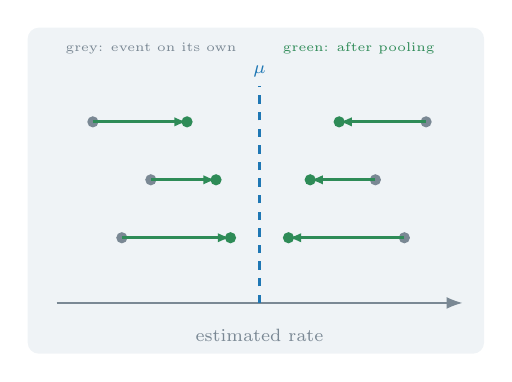
\begin{tikzpicture}[font=\scriptsize,scale=0.92,every node/.style={transform shape}]
\fill[wash,rounded corners] (-0.3,-0.6) rectangle (6.0,3.9);
\node[muted,font=\tiny,anchor=west] at (0.1,3.62) {grey: event on its own};
\node[good,font=\tiny,anchor=west] at (3.1,3.62) {green: after pooling};
\draw[muted,-{Latex[length=2mm]}] (0.1,0.1) -- (5.7,0.1);
\node[muted,font=\scriptsize] at (2.9,-0.35) {estimated rate};
\draw[accent,line width=1.4pt,dashed] (2.9,0.1) -- (2.9,3.1);
\node[accent,font=\scriptsize\bfseries] at (2.9,3.3) {$\mu$};
\foreach \x/\y in {0.6/2.6, 5.2/2.6, 1.4/1.8, 4.5/1.8, 1.0/1.0, 4.9/1.0}
  {\fill[muted] (\x,\y) circle (2.2pt);}
\foreach \x/\xx/\y in {0.6/1.9/2.6, 5.2/4.0/2.6, 1.4/2.3/1.8, 4.5/3.6/1.8, 1.0/2.5/1.0, 4.9/3.3/1.0}
  {\draw[-{Latex[length=1.6mm]},good,line width=1pt] (\x,\y) -- (\xx,\y);
   \fill[good] (\xx,\y) circle (2.2pt);}
\end{tikzpicture}
\end{column}
\end{columns}
\vspace{0.7em}
\begin{center}

\begin{tikzpicture}
\node[draw=accent,line width=1.1pt,rounded corners,fill=accent!6,inner sep=8pt,text width=0.82\textwidth,align=center]
  {\lead{$\sigma$ is estimated too.}\ \ Events differ $\Rightarrow$ $\sigma$ grows, pooling weakens.\\
   Events are alike $\Rightarrow$ $\sigma$ shrinks, pooling strengthens.
   {\color{muted}The data decides.}};
\end{tikzpicture}
\end{center}
\end{frame}

% ---------------------------------------------------------------- 10
\begin{frame}{The whole model on one slide}
\vspace{-0.2em}
\begin{center}
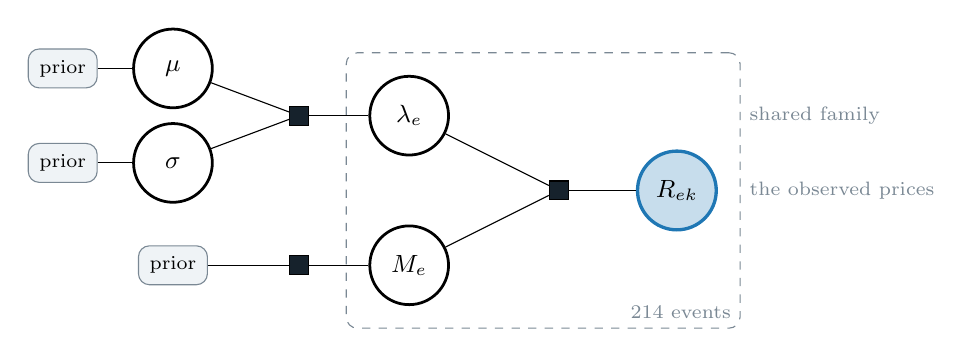
\begin{tikzpicture}[
  font=\small,
  var/.style={circle,draw,line width=1pt,minimum size=10mm,inner sep=0pt},
  obs/.style={circle,draw=accent,line width=1.2pt,fill=accent!25,minimum size=10mm,inner sep=0pt},
  fac/.style={rectangle,draw,fill=ink,minimum size=2.4mm,inner sep=0pt},
  pri/.style={rectangle,draw=muted,rounded corners,fill=wash,inner sep=4pt,font=\scriptsize},
  >={Latex[length=2mm]}]

\node[pri] (pmu) at (0,2.9) {prior};
\node[var] (mu)  at (1.4,2.9) {$\mu$};
\node[pri] (psg) at (0,1.7) {prior};
\node[var] (sg)  at (1.4,1.7) {$\sigma$};
\node[fac] (fp)  at (3.0,2.3) {};
\node[var] (lam) at (4.4,2.3) {$\lambda_e$};

\node[pri] (pa)  at (1.4,0.4) {prior};
\node[fac] (fa)  at (3.0,0.4) {};
\node[var] (amp) at (4.4,0.4) {$M_e$};

\node[fac] (fl)  at (6.3,1.35) {};
\node[obs] (R)   at (7.8,1.35) {$R_{ek}$};

\draw (pmu)--(mu); \draw (psg)--(sg);
\draw (mu)--(fp); \draw (sg)--(fp); \draw (fp)--(lam);
\draw (pa)--(fa); \draw (fa)--(amp);
\draw (lam)--(fl); \draw (amp)--(fl); \draw (fl)--(R);

\begin{scope}[on background layer]
\node[draw=muted,dashed,rounded corners,fit=(lam)(amp)(fl)(R),inner sep=8pt] (pl) {};
\end{scope}
\node[anchor=south east,font=\scriptsize,color=muted] at (pl.south east) {\ 214 events};

\node[anchor=west,font=\scriptsize,color=muted] at (8.6,2.3) {shared family};
\node[anchor=west,font=\scriptsize,color=muted] at (8.6,1.35) {the observed prices};
\end{tikzpicture}
\end{center}
\vspace{0.2em}
\begin{center}
{\color{muted}\small The box repeats per event. Only the shaded node is observed.\\
The link through $\mu,\sigma$ is how one event's data informs another's estimate.}
\end{center}
\end{frame}

% ---------------------------------------------------------------- 11
\begin{frame}{``Isn't there just a formula?''}
\vspace{0.9em}
\begin{center}
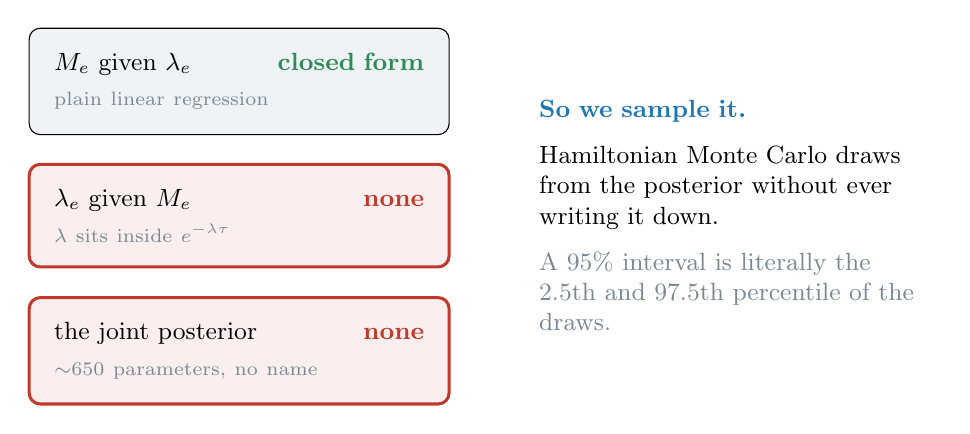
\begin{tikzpicture}[font=\small]
\node[draw,rounded corners,fill=wash,inner sep=9pt,text width=4.7cm,align=left] (a)
  {$M_e$ given $\lambda_e$\hfill\ok{closed form}\\[0.2em]{\color{muted}\scriptsize plain linear regression}};
\node[draw=warn,line width=1.1pt,rounded corners,fill=warn!8,inner sep=9pt,text width=4.7cm,align=left,below=0.35cm of a] (b)
  {$\lambda_e$ given $M_e$\hfill\bad{none}\\[0.2em]{\color{muted}\scriptsize $\lambda$ sits inside $e^{-\lambda\tau}$}};
\node[draw=warn,line width=1.1pt,rounded corners,fill=warn!8,inner sep=9pt,text width=4.7cm,align=left,below=0.35cm of b] (c)
  {the joint posterior\hfill\bad{none}\\[0.2em]{\color{muted}\scriptsize $\sim$650 parameters, no name}};
\node[right=1.0cm of b,text width=5.0cm,align=left] (x)
  {\lead{So we sample it.}\\[0.6em]
   Hamiltonian Monte Carlo draws from the posterior without ever writing it down.\\[0.6em]
   {\color{muted}A 95\% interval is literally the 2.5th and 97.5th percentile of the draws.}};
\end{tikzpicture}
\end{center}
\end{frame}

% ---------------------------------------------------------------- 13
\begin{frame}{What we will report}
\vspace{0.8em}
\begin{columns}[T,onlytextwidth]
\begin{column}{0.31\textwidth}
\centering
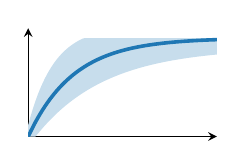
\begin{tikzpicture}[scale=0.85]
\begin{axis}[width=4.4cm,height=3.2cm,axis lines=left,xmin=0,xmax=60,ymin=0,ymax=1.1,
  ytick=\empty,xtick=\empty,tick style={draw=none}]
\addplot[name path=U,draw=none,domain=0:60,samples=80]{min(1,1-exp(-0.12*x)+0.12)};
\addplot[name path=L,draw=none,domain=0:60,samples=80]{max(0,1-exp(-0.045*x)-0.10)};
\addplot[accent!25]fill between[of=U and L];
\addplot[accent,line width=1.3pt,domain=0:60,samples=80]{1-exp(-0.069*x)};
\end{axis}
\end{tikzpicture}\\[0.3em]
{\small\textbf{the curve}}\\{\scriptsize\color{muted}with a 95\% band}
\end{column}
\begin{column}{0.31\textwidth}
\centering
\vspace{0.7em}
{\fontsize{30}{32}\selectfont\bfseries\color{accent}$\tau_{1/2}$}\\[0.6em]
{\small\textbf{one number}}\\{\scriptsize\color{muted}time to get halfway,\\in seconds, with an interval}
\end{column}
\begin{column}{0.31\textwidth}
\centering
\vspace{0.7em}
{\fontsize{30}{32}\selectfont\bfseries\color{accent}$\sigma$}\\[0.6em]
{\small\textbf{is a finding}}\\{\scriptsize\color{muted}large $\sigma$ $\Rightarrow$ there is no\\single speed, only a spread}
\end{column}
\end{columns}
\vspace{1.4em}
\begin{center}
{\color{muted}Plus: is CPI faster than FOMC? Has it changed since 2017?\\Same model, one extra term.}
\end{center}
\end{frame}

% ---------------------------------------------------------------- 14
\begin{frame}{Where it could break}
\vspace{0.5em}
\begin{columns}[T,onlytextwidth]
\begin{column}{0.5\textwidth}
\centering
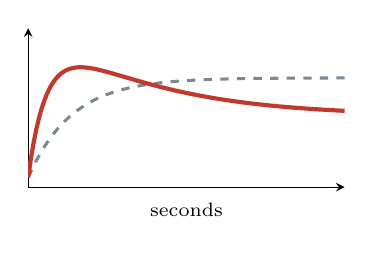
\begin{tikzpicture}
\begin{axis}[width=5.6cm,height=3.6cm,axis lines=left,xmin=0,xmax=60,ymin=-0.1,ymax=1.5,
  xtick=\empty,ytick=\empty,tick style={draw=none},
  xlabel={\scriptsize seconds},label style={font=\scriptsize}]
\addplot[muted,dashed,line width=1.1pt,domain=0:60,samples=80]{1-exp(-0.12*x)};
\addplot[warn,line width=1.5pt,domain=0:60,samples=120]
  {1.35*exp(-0.055*x)*(1-exp(-0.25*x)) + (1-exp(-0.10*x))*0.62};
\end{axis}
\end{tikzpicture}\\[0.2em]
{\scriptsize\color{muted}dashed: what we assume\quad\color{warn}red: overshoot}
\end{column}
\begin{column}{0.46\textwidth}
\vspace{0.6em}
\begin{itemize}\setlength\itemsep{0.65em}\small
\item \bad{Overshoot.} One rate cannot describe a spike that reverts. \lead{Two panels of slide 2 already look like this.}
\item \bad{The hour contains other news.} We cannot separate it.
\item \bad{One venue, one coin.} Binance's clock is Binance's.
\item \bad{FOMC is out.} Powell speaks at 14:30, inside the window.
\end{itemize}
\end{column}
\end{columns}
\vspace{0.5em}
\begin{center}
{\color{muted}\small Full list, in a hostile reviewer's words: \texttt{docs/limitations.md}}
\end{center}
\end{frame}

% ---------------------------------------------------------------- 15
{\setbeamertemplate{footline}{}
\begin{frame}[plain]
\vspace{1.6em}
\begin{center}
{\Large\bfseries The order matters}\\[1.8em]
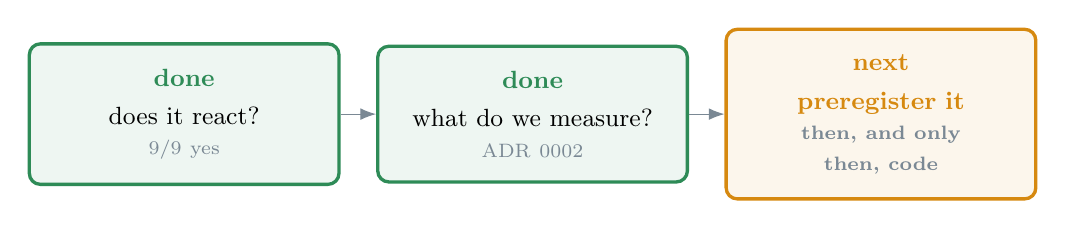
\begin{tikzpicture}[font=\small,node distance=0.45cm]
\node[draw=good,line width=1.2pt,rounded corners,fill=good!8,inner sep=9pt,text width=3.3cm,align=center] (a)
  {\ok{done}\\[0.3em]does it react?\\{\scriptsize\color{muted}9/9 yes}};
\node[draw=good,line width=1.2pt,rounded corners,fill=good!8,inner sep=9pt,text width=3.3cm,align=center,right=of a] (b)
  {\ok{done}\\[0.3em]what do we measure?\\{\scriptsize\color{muted}ADR 0002}};
\node[draw=amber,line width=1.2pt,rounded corners,fill=amber!8,inner sep=9pt,text width=3.3cm,align=center,right=of b] (c)
  {\color{amber}\bfseries next\\[0.3em]preregister it\\{\scriptsize\color{muted}then, and only then, code}};
\draw[-{Latex[length=2mm]},muted] (a)--(b);
\draw[-{Latex[length=2mm]},muted] (b)--(c);
\end{tikzpicture}
\\[2.2em]
{\color{muted}The public commit timestamp proving the plan predates the results\\
is the most valuable thing in this repository.}
\end{center}
\end{frame}}

\end{document}
